%% BEGIN INCLUDE
\documentclass[a4paper, 10pt, twocolumn]{eguk2000}
\usepackage[english]{babel}
\usepackage[square]{natbib}
\usepackage{graphicx}
\usepackage{amsmath}
\usepackage{program}
\usepackage{algorithm}
\usepackage{algorithmicx}
\usepackage{algpseudocode}
\usepackage{hyperref}


\begin{document}
%% END INCLUDE

\title{Screen Space Fluid Rendering with Curvature Flow}
\author{{\sffamily Maarten Terpstra${}^\ast$ and Bram Musters${}^\ast$}\\
\\
${}^\ast$Department of Computing Science\\
University of Groningen\\
Nijenborgh 9\\
Groningen 9747 AG\\
{\tt \{m.l.terpstra, b.t.musters\}@student.rug.nl}\\
\\
\parbox{140truemm}{\normalsize
{\bfseries Abstract}\\
Fluids can be simulated using Smoothed Particle Hydrodynamics(SPH). However, visualizing these fluids in a realistic way proves to be hard.
The paper by \cite{van2009screen} proposes a method that visualizes this SPH simulation as a nature-like fluid using surface smoothing by screen-space curvature flow.
The advantage of this method is that it can be rendered in real-time for a high amount of particles without a need for a finite grid.
This paper analyzes the proposed method and describes how to implement it using C++, OpenGL and the nVidia Cg toolkit.
}
\\
\\
\parbox{140truemm}{\normalsize
{\bfseries Keywords: Smoothed Particle Hydrodynamics, fluid, visualization, computer graphics}
}
} %end author

\date{}


\maketitle 

%!TEX root = ../report.tex
\section{Introduction}
% Sketch the context (what is it all about), what is the application domain (some pictures usually help here). Give required background knowledge.

For some applications it may be useful to simulate fluids using computers in order to improve usage of the fluids in certain situations.
By using visualizations of fluids, bottlenecks or missed opportunities in systems can be identified.
This kind of visualizations are mainly used in engineering.

Other types of visualizations, which are mainly used in academia, includes fields of research as oceanography, volcanology and astrophysics. 
In these kind of visualizations, entire systems are modeled to identify breaking points or how different parameters may affect an entire system.

There are several methods available for simulating fluids, such as the Eulerian method or the Smoothed Particle Hydrodynamics (SPH). The Eulerian method is fairly straightforward, as it describes fluid motion as an integration of the surface over time. 
This simple technique comes with a downside in the fact that it requires a (finite) grid on which the fluid moves, which is computationally expensive and limits the fluid in that it cannot move everywhere.
SPH proves to be a viable alternative. 
With this technique, a body of fluid is reduced to a number of particles, where each particle has a position, velocity, acceleration and density.
These properties can be used to extract a smoothed surface which can then be visualized in an aesthetically pleasing way. 	

Simulating fluids without a visualization may not achieve the desired insight in the system. 
The insight gained from a fluid rendering can be increased by having a natural visualization of the system. 
%!TEX root = ../report.tex
\section{Problem Definition}
% Give a precise formulation of the problem you will be addressing
Since the fluids are simulated using SPH, the fluid is discretized in different particles.
A scene containing a fluid, simulated by SPH, can be seen in figure \ref{..}.
Since this ``fluid'' does not look like a fluid that can be found in nature, a visualization technique has to be applied.

\begin{figure}[!th]
\hrule
\begin{center}
\vspace*{2ex}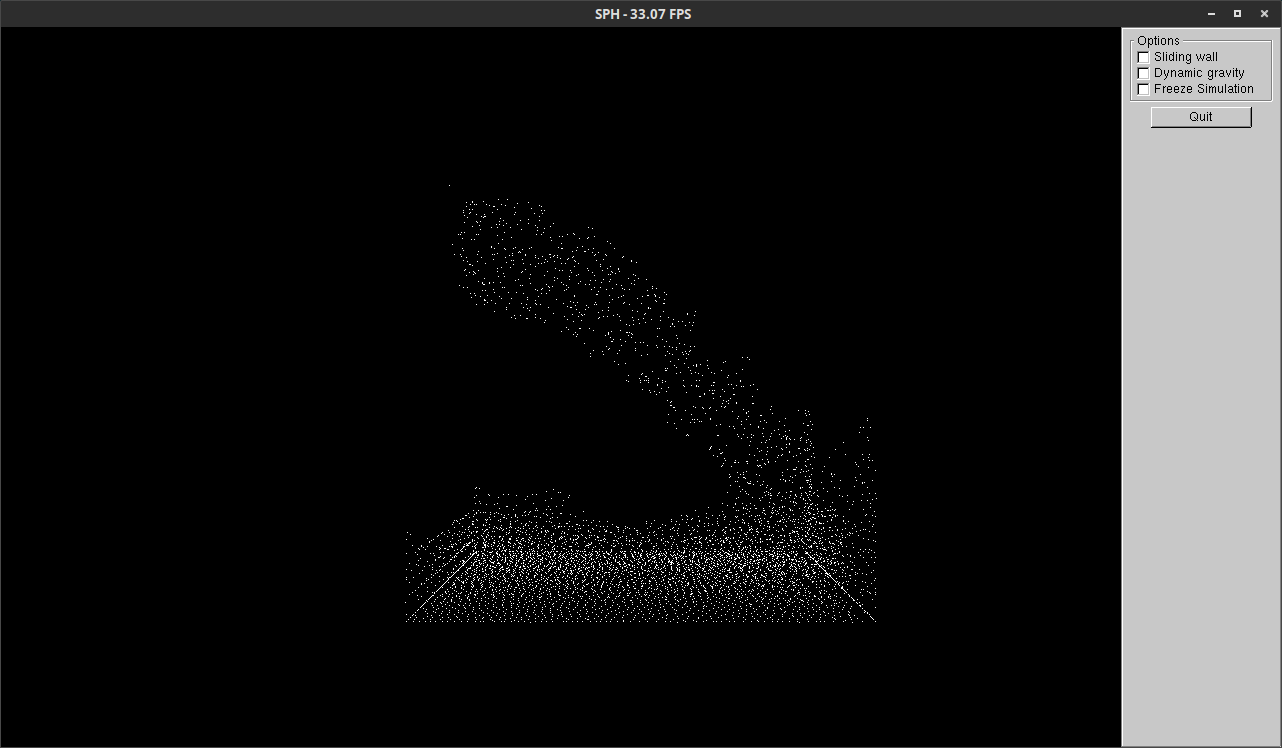
\includegraphics[width=0.48\textwidth]{pictures/sph.png}
\end{center}
\caption{SPH simulation}
\label{fig:sph} 
\vspace*{2ex}
\hrule
\end{figure}

It is our goal to create a nature-like rendering of fluids that can be rendered in real-time, in order to use it in games, for example.
It is also desirable to make sure that the rendering can be customized according to the requirements of users.
For example, fluids can have different kind of thicknesses, or the quality of the rendering can be altered in order to keep the rendering in real-time.

It is also import to distinct what makes a rendering realistic and in real-time. 
We define real-time to be a simulation that is smooth, stutter-free and runs in about the same as the real world.
In practice, this is not always feasible and therefore we define a simulation to be real-time if it produces at least 20 frames per second.

A nature-like visualization of a fluid is a tangible concept as humans have a clear vision of what is a realistic visualization and what is not, but it is not quite as easy to formally define.

There are several components that contribute to a realistic visualization of a fluid.
In order to be realistic a fluid surface needs to be smooth. That is, there are no sharp discontinuities between particles.

Moreover, the surface needs to be imperfect. This may sound counterintuitive as it contradicts with the point that a surface needs to be smooth, but it turns out that in nature a fluid surface is rarely perfectly smooth due to wind and other natural effects.

Finally, a fluid should also act as a fluid in a simulation. This means that object attributes as color should be attenuated as that object is submerged in the fluid and the fluid should produce foam if it is mixed with gases in large quantities. Also, the color of the fluid should change depending on the speed of the fluid.

The combinations of these components are what can make a fluid surface visualization realistic and it these components we seek.
\subsection{Related work}
Various methods are developed that try to achieve a nature-like rendering of fluid.
Some of these techniques require to use a mesh, which is not desirable.
Other techniques have the drawback that they can not be rendered in real-time.

\cite{zhang2008adaptive} developed a method that makes use of point-based rendering, therefore no grid is needed anymore.
However, a drawback of this method is that it results in unreasonably thick surfaces.

%!TEX root = ../report.tex
\section{Solution}
The paper introduced by van der Laan et al. \cite{van2009screen} provides a fitting solution to our problem.
The paper describes a method for visualizing fluids simulated using SPH in a natural way.
The goal of the paper is to provide a solution to our aforementioned problem.
According to the paper, they want to create:
\begin{enumerate}
	\item \label{en:item1} Achieves real-time performance, with a configurable speed versus quality trade-off.
	\item \label{en:item2} Does all the processing, rendering and shading steps directly on the graphics hardware.
	\item \label{en:item3} Smooths the surface to prevent the fluid from looking blobby or jelly-like.
	\item \label{en:item4} Is not based on polygonization, and thus does not suffer from the associated tessellation artifacts.
\end{enumerate}

Items \ref{en:item1} and \ref{en:item3} have a direct connection with our goals and items \ref{en:item2} and \ref{en:item4} are ways to enable these goals.

The method described in the paper consists of multiple passes. It assumes that there is a functional SPH simulation where each fluid particle has a density. Then each frame the following steps are performed:
\begin{enumerate}
	\item Splat points as spheres and determine depth values per fragment
	\item Smooth the spheres based on curvature flow
	\item Attenuate colors based on thickness
	\item Add noise texture and advect throughout the simulation
	\item Add foam
	\item Render using Fresnel and Phong equations
\end{enumerate}

\subsection{Depth determination}
It is desirable to determine depth of fragment in the simulation in order to know which fragments are part of the surface. 
In order to obtain these depth values, the points from the SPH simulation are splatted to discs and their fragments are subjected to a hardware depth test. 
This result is subsequently written to a depth buffer. 
Note that merely the depth value is splatted and the color and normal attributes are left unchanged as they will be changed in later steps.

\subsection{Smoothing}
Smoothing is a critical component in the paper. It is responsible for creating a smooth surface from a set of points so to avoid a blobby and jelly-like surface which is undesirable. The paper argues that this is a better approach than using Gaussian blurring because it performs better and ought to produce better results because there will be no silhouette blurring. 
This is achieved by translating points along the $z$-axis according the curvature flow. 

Curvature flow is defined by the divergence of the normal by \(2H = \nabla \cdot \hat{\mathbf{n}}\). Subsequently, depth values can be displaced every timestep based on the curvature in that point, as \(\frac{\partial z}{\partial t} = H\).

To obtain normals, the point of which the normal needs to be determined is mapped back to a point in view by inverting the projection transformation. This point is called % $\mathbf{P} = \Colvec[;]{a;b;c} $
$\Colvec{a}\Colvec{a,b}\Colvec[;]{a;b;c}$


\subsection{Thickness}

\subsection{Noise}

\subsection{Foam}

\subsection{Rendering}

\subsection{Fit}
%!TEX root = ../report.tex
\section*{Implementation}


%!TEX root = ../report.tex
\section*{Results}


\section{Workload division}
All the programming was done in pairs so we'd value that the programming was 50-50 effort.

For the report, Bram focused more on problem definition, and implementation while Maarten focused more on the solution as proposed by the paper and the introduction.

All in all, we feel that we both contributed equally to the entire final project.


%% BEGIN INCLUDE
\bibliographystyle{eguk2000}
\bibliography{references}
\end{document}
%% END INCLUDE
